\documentclass[12pt]{article}

\usepackage{fancyhdr}
\usepackage{extramarks}
\usepackage{amsmath}
\usepackage{amsthm}
\usepackage{amssymb}
\usepackage{amsfonts}
\usepackage{tikz}
\usepackage[plain]{algorithm}
\usepackage{algpseudocode}
\usepackage{graphicx}

\usetikzlibrary{automata,positioning}

%
% Basic Document Settings
%

\topmargin=-0.45in
\evensidemargin=0in
\oddsidemargin=0in
\textwidth=6.5in
\textheight=9.0in
\headsep=0.25in

\linespread{1.1}

\pagestyle{fancy}
\lhead{\hmwkAuthorName}
\chead{\hmwkClass\ \hmwkTitle}
\rhead{\firstxmark}
\lfoot{\lastxmark}
\cfoot{\thepage}

\renewcommand\headrulewidth{0.4pt}
\renewcommand\footrulewidth{0.4pt}

\setlength\parindent{0pt}

%
% Create Problem Sections
%

\newcommand{\enterProblemHeader}[1]{
    \nobreak\extramarks{}{Problem \arabic{#1} continued on next page\ldots}\nobreak{}
    \nobreak\extramarks{Problem \arabic{#1} (continued)}{Problem \arabic{#1} continued on next page\ldots}\nobreak{}
}

\newcommand{\exitProblemHeader}[1]{
    \nobreak\extramarks{Problem \arabic{#1} (continued)}{Problem \arabic{#1} continued on next page\ldots}\nobreak{}
    \stepcounter{#1}
    \nobreak\extramarks{Problem \arabic{#1}}{}\nobreak{}
}

\setcounter{secnumdepth}{0}
\newcounter{partCounter}
\newcounter{homeworkProblemCounter}
\setcounter{homeworkProblemCounter}{1}
\nobreak\extramarks{Problem \arabic{homeworkProblemCounter}}{}\nobreak{}

%
% Homework Problem Environment
%
% This environment takes an optional argument. When given, it will adjust the
% problem counter. This is useful for when the problems given for your
% assignment aren't sequential. See the last 3 problems of this template for an
% example.
%
\newenvironment{homeworkProblem}[1][-1]{
    \ifnum#1>0
        \setcounter{homeworkProblemCounter}{#1}
    \fi
    \section{Problem \arabic{homeworkProblemCounter}}
    \setcounter{partCounter}{1}
    \enterProblemHeader{homeworkProblemCounter}
}{
    \exitProblemHeader{homeworkProblemCounter}
}

%
% Homework Details
%   - Title
%   - Date
%   - Class
%   - Instructor
%   - Author
%

\newcommand{\hmwkTitle}{Homework\ \#11}
\newcommand{\hmwkDate}{2017-05-20}
\newcommand{\hmwkClass}{MATH6222}
\newcommand{\hmwkClassInstructor}{Instructor: Dr. David Smyth}
\newcommand{\hmwkTutor}{Tutor: Mark Bugden (Wednesday 1-2pm)}
\newcommand{\hmwkAuthorName}{\textbf{Rui Qiu u6139152}}

%
% Title Page
%

\title{
    \vspace{2in}
    \textmd{\textbf{\hmwkClass:\ \hmwkTitle}}\\
    \normalsize\vspace{0.1in}\small{\hmwkDate}\\
    \vspace{0.1in}\large{\textit{\hmwkClassInstructor}}\\
    \vspace{0.1in}
    	\large{\textit{\hmwkTutor}}
    \vspace{3in}
}

\author{\hmwkAuthorName}
\date{}

\renewcommand{\part}[1]{\textbf{\large Part \Alph{partCounter}}\stepcounter{partCounter}\\}

%
% Various Helper Commands
%

% New QED symbol
\renewcommand{\qedsymbol}{$\blacksquare$}

% Useful for algorithms
\newcommand{\alg}[1]{\textsc{\bfseries \footnotesize #1}}

% For derivatives
\newcommand{\deriv}[1]{\frac{\mathrm{d}}{\mathrm{d}x} (#1)}

% For partial derivatives
\newcommand{\pderiv}[2]{\frac{\partial}{\partial #1} (#2)}

% Integral dx
\newcommand{\dx}{\mathrm{d}x}

% Alias for the Solution section header
\newcommand{\solution}{\textbf{\large Solution}}

% Probability commands: Expectation, Variance, Covariance, Bias
\newcommand{\E}{\mathrm{E}}
\newcommand{\Var}{\mathrm{Var}}
\newcommand{\Cov}{\mathrm{Cov}}
\newcommand{\Bias}{\mathrm{Bias}}

\begin{document}

\maketitle

\pagebreak

\begin{homeworkProblem}
Let $G$ be a simple graph with $n$ vertices.\\

(a) Let $x$ and $y$ be nonadjacent vertices of degree at least $(n+k-2)/2$. Prove that $x$ and $y$ have at least $k$ common neighbors.\\

\textbf{Proof:} Suppose the set of adjacent vertices of $x$ is $X$, similarly $Y$ is the set the of adjacent vertices of $y$. Then $|X\cup Y|\leq n-2$ since $x$ and $y$ are not adjacent, so there are at most $n-2$ vertices ($x,y$ excluded) such that they are adjacent to either $x$ or $y$.\\

We are interested in $|X\cap Y|$, which is equal to

\[|X\cap Y| = |X| + |Y| - |X\cup Y| \geq \frac{n+k-2}{2} + \frac{n+k-2}{2} - (n-2)=k\]

Then we are done.\qed\\

(b) Prove that if every vertex has degree at leaset $\lfloor n/2\rfloor$, then $G$ is connected. Show that this bound is the best possible whenever $n\geq 2$ by exhibiting a disconnected $n$-vertex graph where every vertex has at least $\lfloor n/2\rfloor - 1$ neighbors.\\

\textbf{Proof:} Again we use the assumption of $X, Y$ as sets of adjacent vertices of $x,y$. Since the $|X|\geq \lfloor n/2\rfloor$, $|Y|\geq \lfloor n/2 \rfloor$,

\[|X|+|Y| = \lfloor n/2\rfloor + \lfloor n/2\rfloor \geq n-1\]

(For example, $\lfloor 7/2\rfloor + \lfloor 7/2\rfloor = 7-1=6$.)

Similarly, we follow the idea in part (a):

\[|X\cap Y| = |X| + |Y| - |X\cup Y| \geq (n-1) - (n-2) = 1\]

This can be interpreted as every nonadjacent vertices have at least one common neighbor, i.e. $G$ is connected.\\

If we have a disconnected graph $G'$ with one part of $\lfloor n/2\rfloor$ vertices and one part of $\lceil n/2 \rceil$ vertices, for $n\geq 2$, then although each vertex has at least $\lfloor n/2\rfloor -1$ neighbors, it is still disconnected. (The arithmetic reasoning here is $\lfloor n/2\rfloor -1 < \lfloor n/2\rfloor \leq \lceil n/2 \rceil$.)\qed

\end{homeworkProblem}

\begin{homeworkProblem}
Let $G$ be a connected graph with $m\geq 2$ vertices of odd degrees. (Recall from the previous tutorial that $m$ is even). Prove that the minimum number of trails that together traverse each edge of $G$ exactly once is $m/2$. (Hint: Transform $G$ into a new graph $G'$ by adding edges and/or vertices.)\\
	
\textbf{Proof:} By theorem, a graph $G$ is Eulerian if and only if each vertex has even degree and each edge is reachable from every other. So the $G$ in our problem must be non-Eulerian. Also by corollary, $G$ has an even number of odd-degree vertices, say the number is $m=2n, n\in\mathbb{N}.$\\

Suppose $v_1,v_2,\dots,v_m$ are those vertices with odd degrees, we pair them up to $n$ pairs as $(v_1, v_2), (v_3, v_4), \dots, (v_{m-1}, v_m)$, such that a new graph is formed, and we call it $G'$.\\

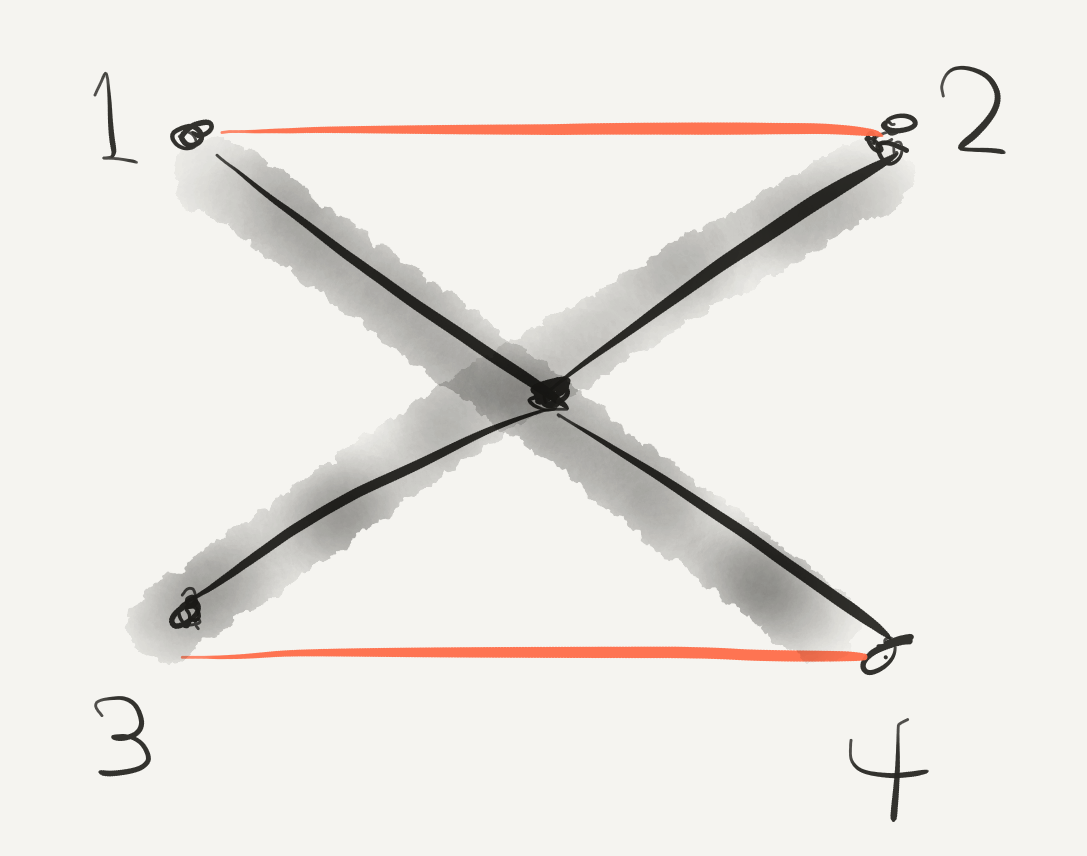
\includegraphics[width=\textwidth]{images/graph}

$G'$ is connected (because $G$ was), and each vertex has an even degrees, by the theorem we used at beginning, $G'$ is Eulerian.\\

Now here comes the tricky part, $G'$ is Eulerian, so whenever we traverse it, we will at some point traverse some edges we added additionally, i.e. not in $E(G)$, but in $G'-E(G)$. So whenever this happens when traversing $G'$ , we count $1$, because if we are now really traversing $G$, we have to ``start'' another trail (or you can consider it as ``jump'' through the artificially added edges).\\

In this way, we have to make $n=m/2$ trails to fully traverse the original graph $G$.\qed 

\end{homeworkProblem}

\begin{homeworkProblem}
Let $G$ be a graph with $n$ vertices and no cycles of length three. Prove that $G$ has at most $n^2/4$ edges. (Hint: Consider the subgraph consisting of neighbors of a vertex of maximum degree and the edges among them.)\\

\textbf{Proof:} Suppose $G$ is a graph with $n$ vertices and no cycles of length $3$. Suppose again that $v_0\in G$ is the vertex with maximum degree $k$. We call the neighbors of $v_0$, $\{v_1,v_2,\dots, v_k\}$. We have to understand that the adjacent vertices of $v_0$ are not adjacent, since otherwise two of those and $v_0$ would form a cycle of length $3$. There are other $n-k-1$ vertices which are not neighbour of $v_0$ (nor itself), if we sum up all the degrees of $n-k-1$ non-neighbors of $v_0$ and the degree of $v_0$, we will have a sum greater or equal to the number of total edges of $G$, which is $e(G)$. In other words,

\[d(v_0)+d(v_{k+1})+\cdots + d(v_{n-1}) \geq e(G)\]

Also, for $v_0, v_{k+1}, v_{k+2},\dots, v_{n-1}$, these $n-k$ vertices, each has at most $k$ degrees. So

\[\begin{split}
	d(v_0)+d(v_{k+1})+\cdots + d(v_{n-1}) &\leq k\cdot(n-k)\\
	e(G) &\leq k(n-k)\\
	e(G) \leq \frac{k+n-k}{2}\cdot\frac{k+n-k}{2} &=\frac{n^2}{4}
\end{split}
\]

Therefore, $G$ has at most $\frac{n^2}{4}$ edges.\qed
\end{homeworkProblem}

\begin{homeworkProblem}
Suppose that every vertex of a graph $G$ has degree at most $k$. Prove that $\chi(G)\leq k+1$. Show that this bound is the best possible by exhibiting (for every $k$) a graph with maximum degree $k$ and chromatic number $k+1$.\\

\textbf{Proof:} We can prove this by induction.\\

Base step: suppose $k=1$, i.e. the maximum degree of a vertex in $G$ is $1$. So $G$ is a path. For a path, $\chi(G)=2\leq 1+1$. So we are done.\\

Inductive hypothesis: suppose $k=n, n\in\mathbb{N}$, the maximum degree of a vertex in $G$ is $n$, and $\chi(G)\leq n+1$.\\

Suppose $G$ is such a graph with maximum degree $n$, now we add a new vertex $v_a$ into $G$, and connect it to the vertex $v_0$ with maximum degree. We consider the worst case, that this $v_a$ is also connected with all other adjacent vertices of $v_0$. In order to differ it from all other adjacent vertices of $v_0$, we cannot use the colors of those adjacent vertices, and we also cannot use the color of $v_0$ because $v_a, v_0$ are adjacent. So we have to use a totally new color for $v_a$, thus increasing the bound of $\chi(G)$ by 1. Therefore, $\chi(G) \leq n+2$ for $k=n+1$.\\

Hence, for every vertex of a graph $G$ with degree at most $k$, $\chi(G)\leq k+1$.\\

Also, if every vertex in $G$ is the ``worst case'' we were talking about above, then $G$ is a complete graph, as $K_{k+1}$, i.e. each vertex is adjacent to all other vertices, all vertices have the same degree $k$, and $\chi(G)=k+1$. And naturally, for any case ``better'' than the worst case, $\chi(G)\leq k+1$.\qed
\end{homeworkProblem}

%
% Non sequential homework problems
%

% Jump
%\begin{homeworkProblem}[5]

%\end{homeworkProblem}

\end{document}
